%%%%%%%%%%%%%%%%%%%%%%%%%%%%%%%%%%%%%%%%%
% Short Sectioned Assignment LaTeX Template Version 1.0 (5/5/12)
% This template has been downloaded from: http://www.LaTeXTemplates.com
% Original author:  Frits Wenneker (http://www.howtotex.com)
% License: CC BY-NC-SA 3.0 (http://creativecommons.org/licenses/by-nc-sa/3.0/)
%%%%%%%%%%%%%%%%%%%%%%%%%%%%%%%%%%%%%%%%%

%----------------------------------------------------------------------------------------
%	PACKAGES AND OTHER DOCUMENT CONFIGURATIONS
%----------------------------------------------------------------------------------------

\documentclass[paper=a4, fontsize=11pt]{scrartcl} % A4 paper and 11pt font size

% ---- Entrada y salida de texto -----

\usepackage[T1]{fontenc} % Use 8-bit encoding that has 256 glyphs
\usepackage[utf8]{inputenc}

% ---- Idioma --------

\usepackage[spanish, es-tabla]{babel} % Selecciona el español para palabras introducidas automáticamente, p.ej. "septiembre" en la fecha y especifica que se use la palabra Tabla en vez de Cuadro

% ---- Otros paquetes ----

% Hipervínculos
\usepackage[hidelinks]{hyperref}

\usepackage{amsmath,amsfonts,amsthm} % Math packages
\usepackage{graphics,graphicx, float, url} %para incluir imágenes y colocarlas
\usepackage{ulem}

\usepackage{fancyhdr} % Custom headers and footers
\pagestyle{fancyplain} % Makes all pages in the document conform to the custom headers and footers
\fancyhead{} % No page header - if you want one, create it in the same way as the footers below
\fancyfoot[L]{} % Empty left footer
\fancyfoot[C]{} % Empty center footer
\fancyfoot[R]{\thepage} % Page numbering for right footer
\renewcommand{\headrulewidth}{0pt} % Remove header underlines
\renewcommand{\footrulewidth}{0pt} % Remove footer underlines
\setlength{\headheight}{13.6pt} % Customize the height of the header

\numberwithin{equation}{section} % Number equations within sections (i.e. 1.1, 1.2, 2.1, 2.2 instead of 1, 2, 3, 4)
\numberwithin{figure}{section} % Number figures within sections (i.e. 1.1, 1.2, 2.1, 2.2 instead of 1, 2, 3, 4)
\numberwithin{table}{section} % Number tables within sections (i.e. 1.1, 1.2, 2.1, 2.2 instead of 1, 2, 3, 4)

\setlength\parindent{0pt} % Removes all indentation from paragraphs - comment this line for an assignment with lots of text

\newcommand{\horrule}[1]{\rule{\linewidth}{#1}} % Create horizontal rule command with 1 argument of height

%----------------------------------------------------------------------------------------
%	TÍTULO Y DATOS DEL ALUMNO
%----------------------------------------------------------------------------------------

\title{	
\normalfont \normalsize 
\textsc{{\bf Ingeniería de Servidores (2015-2016)} \\ Doble Grado en Ingeniería Informática y Matemáticas \\ Universidad de Granada} \\ [25pt] % Your university, school and/or department name(s)
\horrule{0.5pt} \\[0.4cm] % Thin top horizontal rule
\huge Memoria Práctica 2 \\ % The assignment title
\horrule{2pt} \\[0.5cm] % Thick bottom horizontal rule
}

\author{Óscar Bermúdez Garrido\\ \href{http://www.github.com/oxcar103}{@oxcar103}} % Nombre y apellidos

\date{\normalsize\today} % Incluye la fecha actual

%----------------------------------------------------------------------------------------
% DOCUMENTO
%----------------------------------------------------------------------------------------

\begin{document}
\maketitle % Muestra el Título
\newpage %inserta un salto de página
\tableofcontents % para generar el índice de contenidos
\listoffigures

\begin{enumerate}
	\section{Instalación de servicios y configuración}
	\subsection{yum}
		\item Liste los argumentos de yum necesarios para instalar, buscar y eliminar paquetes.
		
		Basado en \cite{man_yum}:
		
		\textbf{Para instalar:} \textit{sudo yum install $<$paquete$>$}, por ejemplo: \textit{sudo yum
		install oneko}.
		
		\textbf{Para buscar:} \textit{yum search $<$expresión$>$}, por ejemplo: \textit{yum search sl}.
		
		\textbf{Para eliminar:} \textit{sudo yum remove $<$paquete$>$}, por ejemplo: \textit{sudo yum
		remove bsd-games}.
		
		
		\item ¿Qué ha de hacer para que yum pueda tener acceso a Internet?\footnote{Pista: archivo de
		configuración en /etc, proxy: stargate.ugr.es:3128} ¿Cómo añadimos un nuevo repositorio?
		
		Para hacer que yum pueda acceder a Internet a través de un proxy, debemos modificar el archivo
		\textit{/etc/yum/yum.conf}, con el comando \textit{nano} por ejemplo, y añadir la variable
		\textit{proxy} con el valor del proxy(en este caso, \textit{stargate.ugr.es:3128}) como podemos
		ver en \cite{man_yum.conf}, \cite{CentOS_web} y \cite{foro_Fedora}.
		
		Para añadir nuevos repositorios podemos instalar el paquete \textit{yum-utils} y añadir nuevos
		repositorios usando el comando \textit{yum-config-manager} tal y como nos indica su propio
		manual \cite{man_yum-config-manager}. O podemos incluir directamente la dirección del repositorio
		en \textit{/etc/yum/yum.conf} como se indica en \cite{man_yum.conf}.
	
	\subsection{apt}
		\item Indique el comando para buscar un paquete en un repositorio y el correspondiente para
		instalarlo.
		
		Basado en \cite{man_apt-cache} y \cite{man_apt-get}:
		
		\textbf{Para buscar:} \textit{apt-cache search $<$expresión$>$}, por ejemplo: \textit{apt-cache
		search sl}.
		
		\textbf{Para instalar:} \textit{sudo apt-get install $<$paquete$>$}, por ejemplo: \textit{sudo
		apt-get install oneko}.
		
		\textbf{Para eliminar:} \textit{sudo apt-get remove $<$paquete$>$}, por ejemplo: \textit{sudo
		apt-get remove bsd-games}.
		
		\item Indique qué ha modificado para que apt para acceder a los servidores de paquetes a través
		de proxy. ¿Cómo añadimos un nuevo repositorio?
		
		Para hacer que apt pueda acceder a Internet a través de un proxy, debemos modificar el archivo
		\textit{/etc/apt/apt.conf}, con el comando \textit{nano} por ejemplo, y añadir la variable
		\textit{http\_proxy} con el valor del proxy(en este caso, \textit{stargate.ugr.es:3128}) como
		podemos ver en \cite{man_apt.conf}.
		
		Para añadir nuevos repositorios podemos usar el comando \textit{add-apt-repository} tal y como
		nos indica su propio manual \cite{man_add-apt-repository}. O podemos incluir directamente la
		dirección del repositorio en \textit{/etc/apt/sources.list} ya que en \cite{man_apt} se indica
		que utilicemos \textit{apt edit-sources} para este propósito pero lo único que hace este comando
		es abrirnos el archivo antes citado para su edición.
	
	\subsection{Windows}
	\subsection{openSUSE}
		\item ¿Qué gestores utiliza openSUSE?\footnote{Pista: \url{http://es.opensuse.org/Gestión_de_paquetes}}
		
		Como podemos ver en \cite{oS_packman}, de forma nativa openSUSE utiliza dos gestores de paquetes:
		
		\begin{itemize}
			\item \textbf{YaST}\cite{oS_YaST}(\textit{Yet another Setup Tool}) para la gestión de manera
			gráfica.
			\item \textbf{Zypper}\cite{oS_zypper} para la gestión por línea de comandos.
		\end{itemize}
		
		De hecho, ambos servicios están colgados de forma abierta y permitiendo no sólo ver el código
		que utilizan si no también proponer cómo corregir un bug encontrado, reportarlo o simplemente
		crear nuestro propio gestor de paquetes basado en alguno de ellos\cite{oS_YaST_GitHub}
		\cite{oS_zypper_GitHub}.
		
		Ambos se distribuyen bajo la licencia \href{https://www.gnu.org/licenses/gpl.html}{\textbf{GPL}}
		\footnote{De hecho, creo que incluso utilizan la misma versión de dicha licencia.}.
	
	\section{Gestión de los cortafuegos(\textit{Firewalls})}
	\section{Instalación del servicio de acceso remoto a la consola(\textit{Secure Shell})}
		\item ¿Qué diferencia hay entre telnet y ssh?
		
		La principal diferencia entre ambos protocolos de red es la seguridad\cite{Telnet}\cite{SSH}.
		De hecho, SSH se diseñó para reemplazar a algunos protocolos de red como Telnet mediante
		la solución del problema que tenía estos protocolos, que era que no ofrecían confidencialidad
		en redes poco seguras como las redes públicas y podían ser atacados por terceras personas
		conectadas a dicha red. SSH para solucionarlo, encripta los datos.
	
		\item ¿Para qué sirve la opción \textbf{-X}? Ejecute remotamente, es decir, desde la máquina
		anfitriona (si tiene Linux) o desde la otra máquina virtual, el comando \textit{gedit} en una
		sesión abierta con \textit{ssh}. ¿Qué ocurre?
		
		Como podemos ver en \cite{man_SSH}, este parámetro nos permite la ejecución de aplicaciones
		que utilicen el entorno gráfico durante una sesión abierta de \textit{secure shell} como si
		se estuviera ejecutando directamente sobre la máquina, esto es, todos los cambios se producen
		en ella con la diferencia de que no es necesario tener un entorno gráfico instalado en la
		misma pues se ejecuta sobre la máquina que tiene la sesión de \textit{secure shell} abierta.
		
		Si no fuese posible dicha conexión(pero sí la conexión \textit{ssh}), nos informa que no es
		posible la ejecución de este parámetro pero establece la sesión de forma normal.
		
		\item Muestre la secuencia de comandos y las modificaciones a los archivos correspondientes
		para permitir acceder a la consola remota sin introducir la contraseña\footnote{Pista: ssh-keygen,
		ssh-copy-id}.
		
		Primero, configuramos el acceso para que sea posible desde el host, como se nos indica en
		\cite{SSH_StackOverFlow}.
		
		Después, ejecutamos \textit{ipconfig} para ver nuestra IP y la del dispositivo que queremos
		conectar:
		
		\begin{figure}[H]
			\centering
			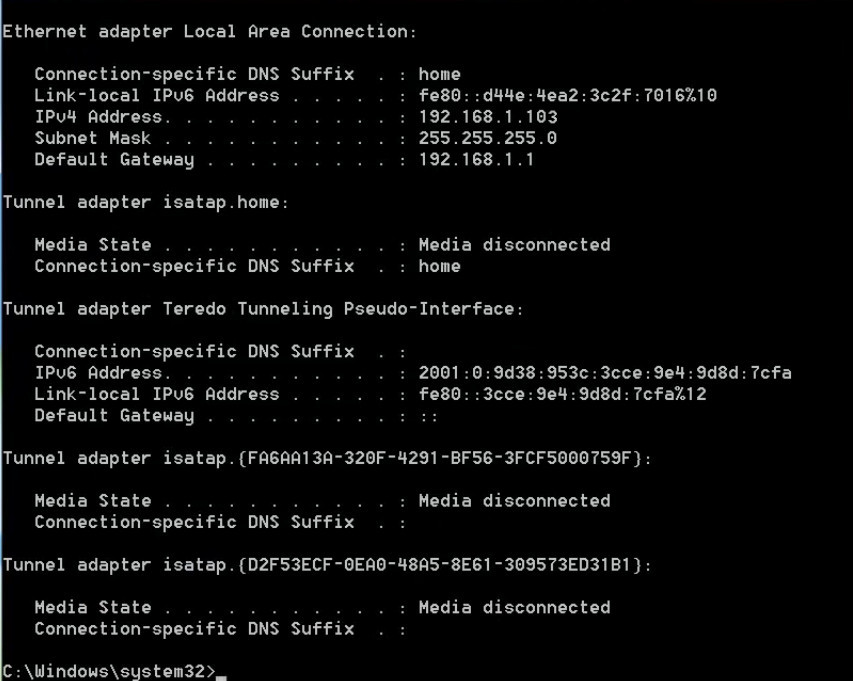
\includegraphics[width=15cm]{Ejercicio_8a.jpg}
			\caption{Tabla de direcciones generada por \textit{ipconfig}.}
			\label{fig:ipconfig}	
		\end{figure}
		
		La nuestra sería \textbf{192.168.1.103} y la de Ubuntu Server,\textbf{192.168.1.101}.
		
		Una vez, hecho esto, intentamos acceder por ssh y ejecutamos \textit{ifconfig} para ver que
		efectivamente, estamos dentro, como se ve en la siguiente captura:
		
		\begin{figure}[H]
			\centering
			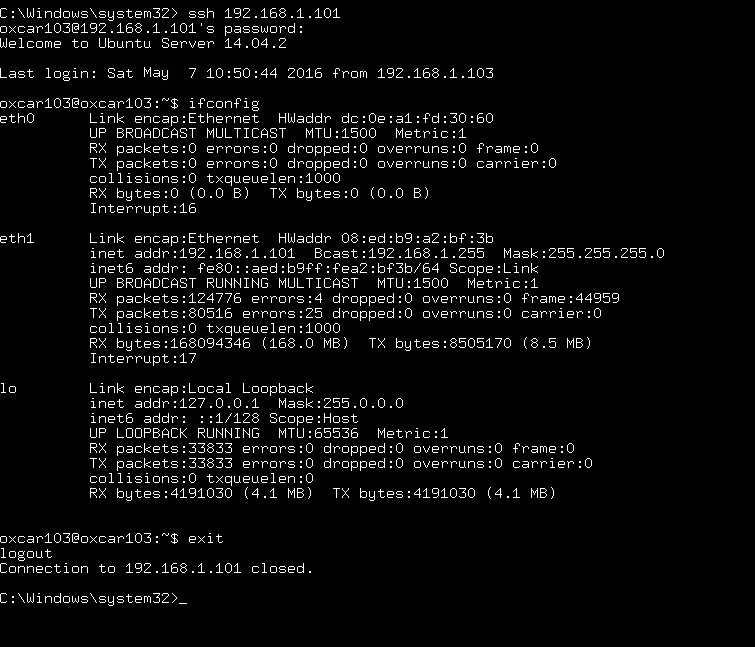
\includegraphics[width=15cm]{Ejercicio_8b.jpg}
			\caption{Prueba del funcionamiento de \textit{ssh} sin clave}
			\label{fig:test_1}	
		\end{figure}
		
		Ahora, usando el comando \textit{ssh-keygen} \cite{man_ssh-keygen}, generaremos un par de
		claves pública-privada en Ubuntu Server. En los archivos \textit{id\_rsa} y \textit{id\_rsa.pub}
		\footnote{Nótese que el nombre del archivo se puede cambiar como bien se indica en
		\cite{man_ssh-keygen}.} quedará registrada la clave pública que se usará para conectar con
		Ubuntu Server, estos archivos los llevaremos al sistema operativo host. Para ello, usaremos
		\textit{ssh-copy-id} \cite{man_ssh-copy-id}.
		
		El proceso y el resultado(una conexión sin pedir la contraseña), se puede ver en la imagen:
		
		\begin{figure}[H]
			\centering
			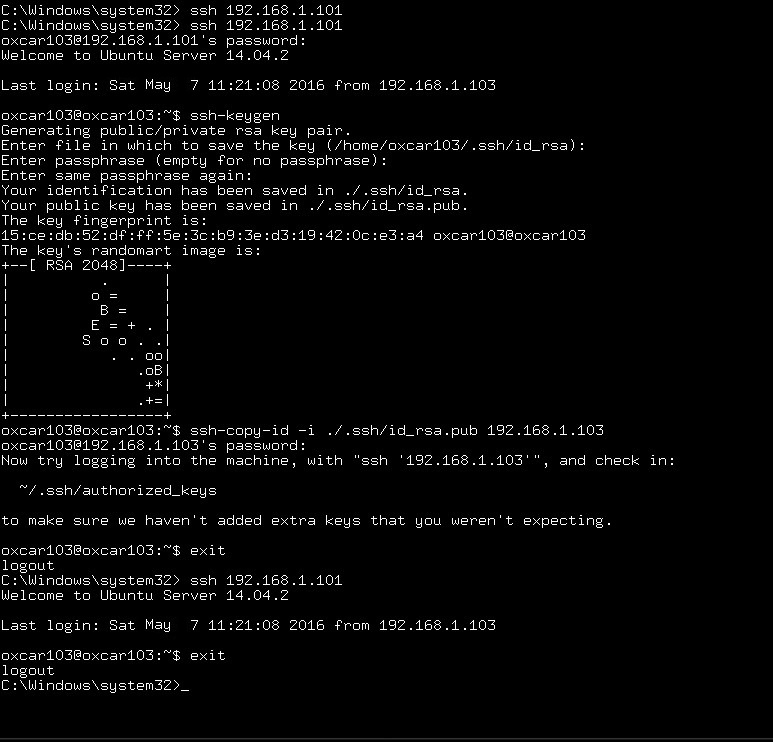
\includegraphics[width=15cm]{Ejercicio_8c.jpg}
			\caption{Prueba del funcionamiento de \textit{ssh} con clave.}
			\label{fig:test_2}	
		\end{figure}
		
		\item ¿Qué archivo es el que contiene la configuración de sshd? ¿Qué parámetro hay que modificar
		para evitar que el usuario root acceda? Cambie el puerto por defecto y compruebe que puede
		acceder.
		
		El archivo de configuración que buscábamos es \textit{sshd\_config}\cite{man_sshd_config}, en
		el cuál podremos gestionar de forma más sencilla cada uno de los parámetros de dicho
		\textit{daemon}
		
		Primero, comprobamos que nos podemos conectar:
		
		\begin{figure}[H]
			\centering
			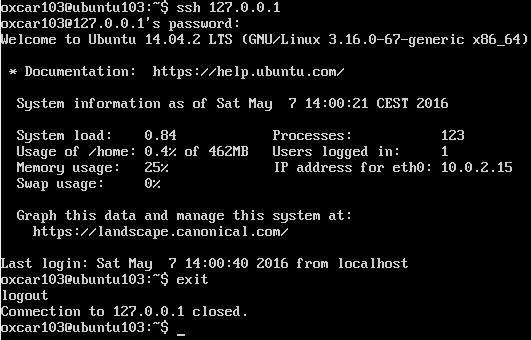
\includegraphics[width=15cm]{Ejercicio_9a.jpg}
			\caption{Entramos a \textit{ssh} por el puerto por defecto.}
			\label{fig:before}	
		\end{figure}
		
		Ahora, cambiamos los parámetros que consideremos oportunos con un editor, por ejemplo,
		\textit{nano}\cite{man_nano} en el cuál sólo cambiaremos el puerto por defecto esta vez:
		
		\begin{figure}[H]
			\centering
			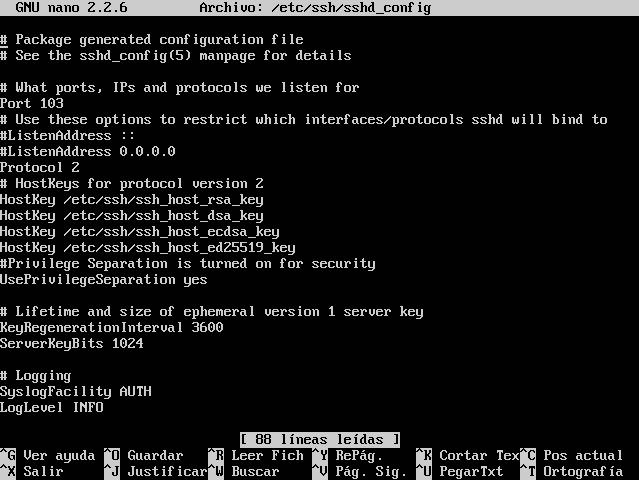
\includegraphics[width=15cm]{Ejercicio_9b.jpg}
			\caption{Archivo de configuración modificado.}
			\label{fig:edit}	
		\end{figure}
		
		Tras esto, es necesario reiniciar el servicio.
		
		Finalmente, vemos que al intentar entrar por \textit{ssh} al puerto por defecto, nos da un
		error, mientras que si intentamos entrar por el nuevo puerto, se nos permite la entrada tras
		escribir correctamente la contraseña:
		
		\begin{figure}[H]
			\centering
			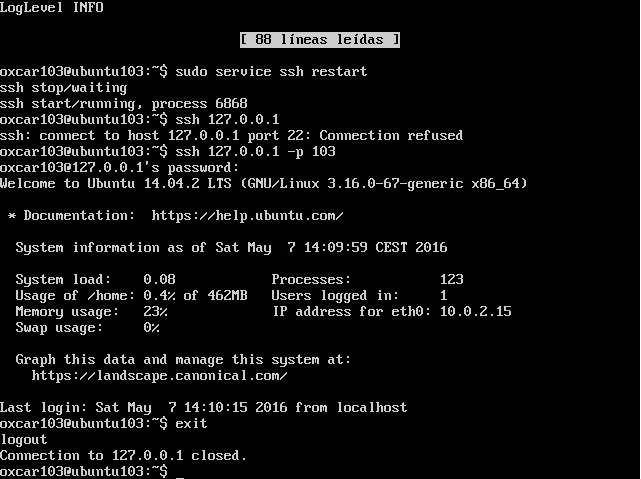
\includegraphics[width=15cm]{Ejercicio_9c.jpg}
			\caption{Comprobación de que surtió efecto el cambio.}
			\label{fig:after}	
		\end{figure}
		
		\item Indique si es necesario reiniciar el servicio. ¿Cómo se reinicia un servicio en Ubuntu?
		¿Y en CentOS? Muestre la secuencia de comandos para hacerlo.
		
		Utilizando el comando \textit{apropos}\cite{man_apropos}, podemos encontrar que los gestores
		por defecto para la gestión de servicios son \textit{service}\cite{man_service} en Ubuntu Server
		y \textit{systemctl}\cite{man_systemctl} para CentOS, ambos con una sintaxis similar:
		
		\begin{itemize}
			\item \textit{sudo systemctl <acción> <servicio>}
			\item \textit{sudo service <servicio> <acción>}
		\end{itemize}
		donde la acción puede ser \textit{start}, \textit{stop} o \textit{restart} entre otras.
		
		Por supuesto, otra forma perfectamente válida es ejecutar directamente el script específico del
		servicio, sin embargo, para ello hay que saber dónde está ubicado.
		
	
	\subsection{Utilidades: screen y terminator}
		\item Instale y pruebe \textit{terminator}. Con \textit{screen}, pruebe su funcionamiento
		dejando sesiones \textit{ssh} abiertas en el servidor y recuperándolas posteriomente.
	
	\subsection{Un poco de seguridad: \textit{fail2ban}}
		\item Instale el servicio y pruebe su funcionamiento.
		
		Para instalarlo, utilizaremos cualquiera de los gestores de paquetes que hemos visto
		anteriormente.
		
		Posteriormente, accederemos a \cite{man_fail2ban}, donde podremos ver que podemos modificar
		el comportamiento del servicio tanto a nivel de cliente como de servidor. Entre otros archivos
		de configuración en \textit{jail.conf}\cite{man_jail.conf} podemos configurar las restricciones
		que queremos adoptar frente a cada servicio que supervisa, dando por ejemplo a ssh un máximo
		de 3 intentos antes de banear la ip y en el resto de servicios ponerlo a 5. Incluso podemos
		definir reglas en la carpeta \textit{filter.d} restringiendo la hora de acceso a ciertos
		servicios o baneando ciertas direcciones MAC.
		
	\section{Administración remota de Windows}
	\section{Instalación de un servidor web básico}
	\subsection{Instalación de Apache + MySQL (o MariaDB) + PHP (o Python) en Linux(\textit{LAMP})}
		\item Muestre los comandos que ha utilizado en Ubuntu Server y en CentOS (aunque en este último
		puede utilizar la GUI; en tal caso, realice capturas de pantalla).
		
		Para el caso de Ubuntu, instalaremos el servicio como un pack usando el comando \textit{sudo
		apt-get install lamp-server\^}.
		
		Para CentOS, lo instalaremos componente a componente para mostrar ambos métodos, es decir:
		\begin{itemize}
			\item \textit{httpd} para instalar el servicio Apache, lo añadiremos a la lista de
			ejecuciones durante el arranque con \textit{systemctl enable httpd.service}.
			
			\item \textit{mariadb} para la base de datos de Maria-DB\footnote{Originalmente, la base
			de datos a la que hace referencia es \textit{MySQL} pero hace algún tiempo, tomó fuerza la
			base de datos alternativa de \textit{Maria-DB}}
			
			\item \textit{php} y \textit{php-mysql} para el servidor PHP.
		\end{itemize}
		
		Por último, en ambos sistemas operativos reiniciaremos los servicios para asegurarnos que los
		cambios de configuración que se produjeron durante la instalación de los mismo surte efecto
		\footnote{Sería conveniente incluir el servicio de Apache para que sea capaz de atravesar el
		cortafuegos al tratarse de un servicio web}.
		
		\item Enumere otros servidores web y las páginas de sus proyectos (mínimo 3 sin considerar
		Apache, IIS ni nginx).
		
		Dentro de los servidores web, destacaré los que ya estudié en otro proyecto similar\cite{TWG}:
		\begin{itemize}
			\item \textbf{Apache Tomcat}\cite{TC_official}(también llamado simplemente Tomcat), que
			en la página oficial se nos describe como un contenedor de Servlet y JavaServer Pages
			implementado en Java en código abierto desarrollado por la comunidad de desarrolladores
			de la \textit{Apache Software Foundation (ASF)} bajo la licencia de software libre
			\href{https://www.apache.org/licenses/LICENSE-2.0.html}{\textbf{Apache License 2.0.}}
			
			\item \textbf{JBoss}\cite{WF_official}(Actualmente, llamado \textit{WildFly}), que en la
			página oficial se nos describe como un servidor de aplicaciones implementado en Java en
			código abierto desarrollado por \textit{RedHat} bajo la licencia de software libre
			\href{https://www.gnu.org/licenses/lgpl.html}{\textbf{GNU Lesser General Public License(LGPL)}}.
			
			\item Al igual que WildFly, GlassFish es un servidor de aplicaciones implementado en Java
			en código abierto y desarrollado por \textit{Oracle Corporation} bajo una licencia dual
			\href{https://opensource.org/licenses/CDDL-1.0}{\textbf{Common Development and Distribution
			License (CDDL)}}\footnote{En este enlace, no he usado el oficial, es decir, el de Oracle
			porque me dio la sensación de que dirigía a un archivo temporal pero lo dejo aquí:
			\href{http://www.oracle.com/technetwork/middleware/oedq/help/edq11help-2152391.pdf}{\textbf{CDDL}}}
			\& \href{https://www.gnu.org/licenses/gpl.html}{\textbf{GPL}}
			con una ligera modificación.\cite{GF_official}\cite{GF_install}
		\end{itemize}
		
	\subsection{Windows: IIS}
		\item Compruebe que el servicio está funcionando accediendo a la MV a través de la anfitriona.
		
		Para lograr conectar la máquina anfitriona con la máquina virtual, lo primero que tendremos que
		hacer es asegurarnos que se ven, pero por defecto, Windows Server no permite hacerle ping,
		tenemos que ajustarlo modificando la regla mostrada en la figura:
		
		\begin{figure}[H]
			\centering
			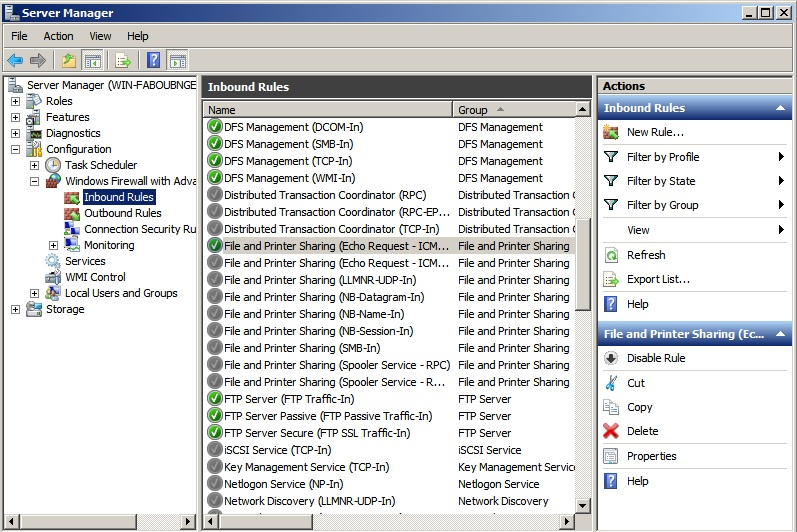
\includegraphics[width=15cm]{Ejercicio_15a.jpg}
			\caption{Activando señal ping.}
			\label{fig:ping}
		\end{figure}
		
		Para la transferencia de un archivo por ftp, necesitamos abrir un puerto para dicho fin,
		utilizaremos el puerto 21 para lo cuál tendremos que modificar en:
		
		\begin{figure}[H]
			\centering
			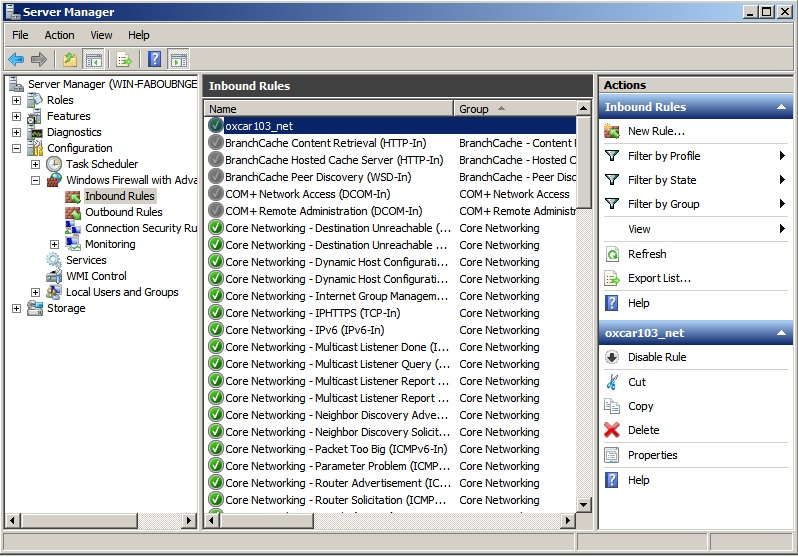
\includegraphics[width=15cm]{Ejercicio_15b.jpg}
			\caption{Abriendo puerto ftp.}
			\label{fig:ftp}
		\end{figure}
		
		Tras esto, necesitamos reinciar el servicio de cortafuegos en la subsección \textit{Services}.
		
		Ahora, crearemos un usuario a través del cuál realizaremos la transferencia:
		
		\begin{figure}[H]
			\centering
			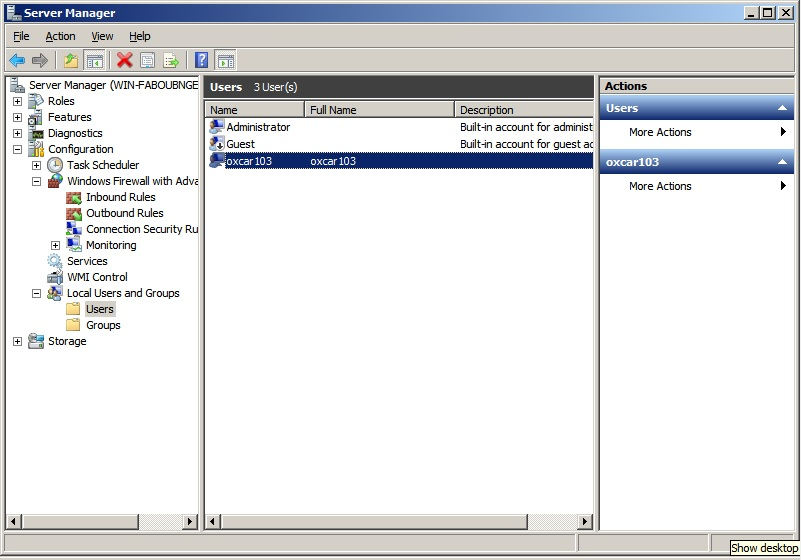
\includegraphics[width=15cm]{Ejercicio_15c.jpg}
			\caption{Creación del nuevo usuario.}
			\label{fig:user}
		\end{figure}
		
		Y también necesitamos un servidor FTP:
		
		\begin{figure}[H]
			\centering
			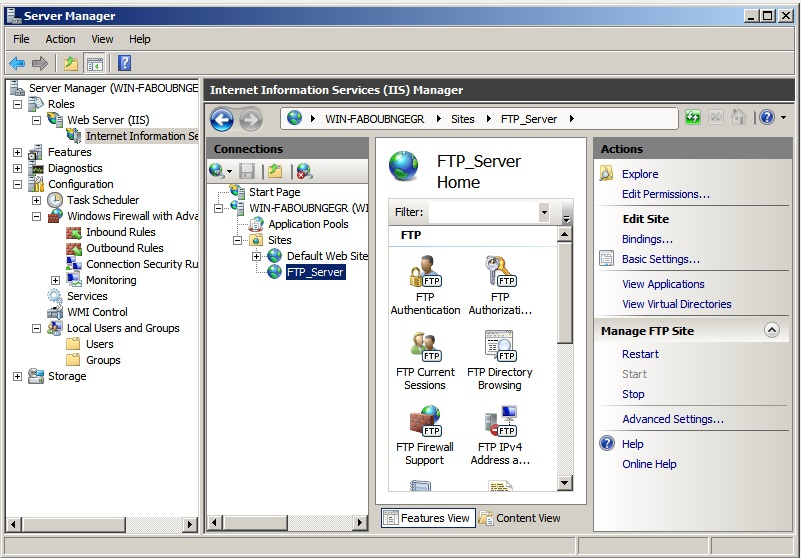
\includegraphics[width=15cm]{Ejercicio_15d.jpg}
			\caption{Configuración del servidor.}
			\label{fig:server}
		\end{figure}
		
		Finalmente, creamos un archivo:
		
		\begin{figure}[H]
			\centering
			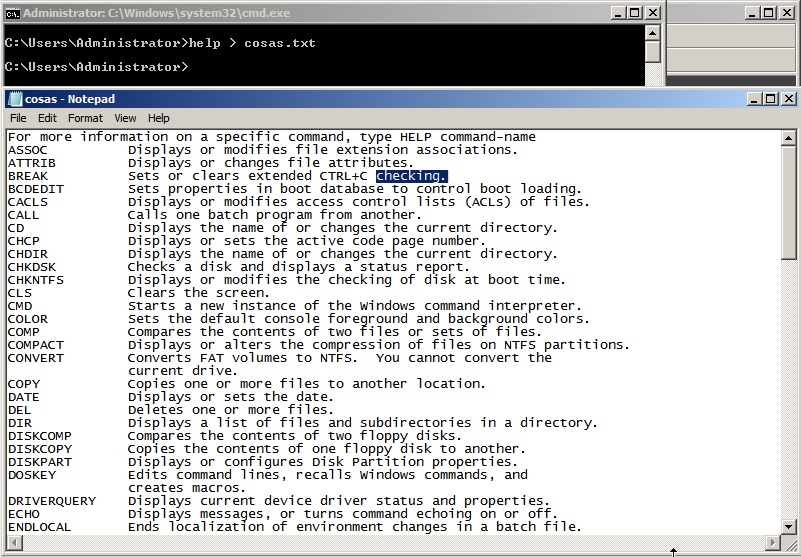
\includegraphics[width=15cm]{Ejercicio_15e.jpg}
			\caption{Archivo a enviar.}
			\label{fig:send}
		\end{figure}
		
		Y lo transferimos:
		
		\begin{figure}[H]
			\centering
			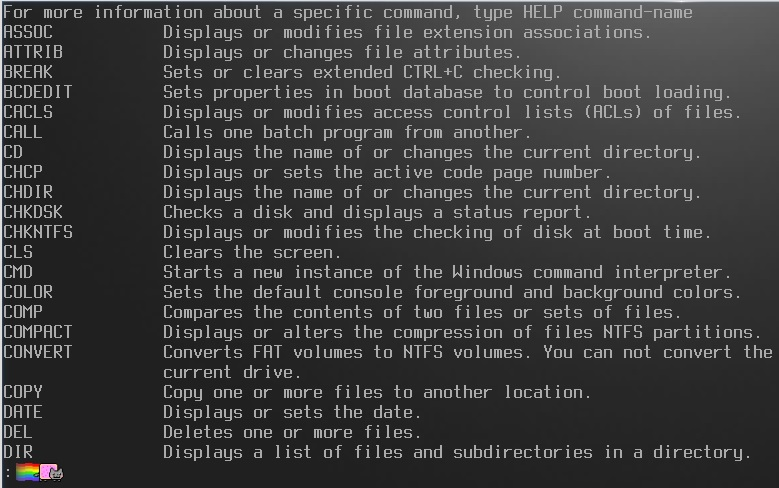
\includegraphics[width=15cm]{Ejercicio_15f.jpg}
			\caption{Archivo transferido.}
			\label{fig:received}
		\end{figure}
		
		
		
	\subsection{Windows y otros servidores web}
	\subsection{Java Servlets}
		\item Realice la instalación de uno de estos dos \textit{web containers} y pruebe su ejecución.
		
		De nuevo, utilizaremos el trabajo realizado en \cite{TWG}\footnote{Por ello, dejaré como
		pruebas del funcionamiento de los servicios las que ya subí para dicho trabajo}:
		
		\begin{itemize}
			\item Instalar Tomcat se puede realizar fácilmente basándonos en las indicaciones dadas
			en \cite{TC_install}:
			
			\begin{itemize}
				\item Nos descargamos de \cite{TC_download} el archivo .zip correspondiente y lo
				descomprimimos donde queramos instalar Tomcat. La instalación acaba satisfactoriamente.
				
				\item Si queremos reubicar el puerto de la página http, Realizaremos los pasos indicados
				en \cite{TC_StackOverFlow}.
				
				\item Y basta con inicializar el servicio ejecutando el script \textit{startup.sh}.
			\end{itemize}
			
			\item Para instalar WildFly seguiremos las instrucciones detalladas en \cite{WF_install}:
			
			\begin{itemize}
				\item Tras haber descargado el archivo adecuado de \cite{WF_download}, descomprimimos
				el archivo en la carpeta deseada.
				
				\item Ahora, para inciar el servicio, bastaría con ejecutar el script
				\textit{standalone.sh} o el script \textit{domain.sh}.
				
				\item La instalación se realiza de una manera correcta pero al intentar ejecutar el
				servicio, se podrían producir una serie de errores que nos impiden dar comienzo al
				servicio\footnote{Como se detalla en \cite{WF_install}, hay otro modo para inicializar
				el servicio, ejecutando \textit{domain.sh} pero igualmente genera una serie de errores
				similares a la ejecución de \textit{standalone.sh}}.
				
				\item En cuyo caso, la solución, podría pasar por utilizar el script proporcionado por
				una página no oficial \cite{WF_solution}\footnote{a pesar de no ser oficial, como he
				podido comprobar que su solución es eficaz, la incluyo como referencia} que, directamente
				descarga un archivo comprimido; posteriormente, lo descomprime e instala en la
				correspondiente carpeta \textit{/opt}; lo configura, modificando así las líneas del
				archivo \textit{standalone.xml} que permite cambiar el puerto por el cual se ofrece el
				servicio y añade el usuario $"$wildfly$"$ automáticamente y activa el servicio.
				
				\item Además, este script en las últimas líneas modificaba el puerto en el cual se da
				el servicio, que puede resultar de utilidad si se va a disponer de varios servidores
				instalados a la vez.
			\end{itemize}
		\end{itemize}
	
	\subsection{Otro tipo de Bases de datos}
		\item Realice la instalación de MongoDB en alguna de sus máquinas virtuales. Cree una colección
		de documentos y haga una consulta sobre ellos
		\footnote{\url{http://docs.mongodb.org/manual/installation/}}.
		% sudo apt-get install mongodb para instalar la base de datos
		% Trabajar con Mongo:
		%	use <Nombre de la base de datos>
		%	show dbs para mostrarla
		%
		%	db.<Nombre DB>.insert{
		%		<Categoría no numérica>: "<valor>",
		%		<Categoría numérica>: <valor>,
		%	}
		%
		%	Buscar "how to query mongodb" en DuckDuckGo
		%
	
	\section{Manteniendo de los servicios actualizados}
		\item Muestre un ejemplo de uso del comando \footnote{\url{http://fedoraproject.org/wiki/VMWare}}
		
		Podemos seguir el ejemplo de la pista del ejemplo o podemos crear nuestro propio ejemplo:
		
		\begin{itemize}
			\item Creamos dos ficheros de texto con algún contenido (sin importar demasiado, pues la
			finalidad del ejercicio es la creación de archivos \textit{.patch} y su aplicación).
			
			\item Una vez creados, mostramos su contenido para que visualmente se pueda hacer la
			comparación.
			
			\item Tras esto, creamos el archivo \textit{.patch} con el comando \textit{diff}
			\footnote{Este comando, tiene parámetros muy interesantes como:
				\begin{itemize}
					\item \textit{-b} para ignorar los espacios en blanco que no suelen ser demasiado
					importantes a la hora de compilar el programa aunque sí a la hora de visualizarlo.
					\item \textit{-N} que en caso de no existir un archivo, lo trata como un archivo vacío.
					\item \textit{-{}-from-file/-{}-to-file} para comparar todos con el archivo(o directorio) % % Para producir -- en lugar de una línea, escribo -{}-
					indicado.
					\item \textit{-r} para comparar recursivamente con los subdirectorios(en caso de que se
					pase como parámetro un directorio).
				\end{itemize}
			}, para más información, se puede visitar \cite{man_diff}.
			
			\item Ahora, basta usar el comando \textit{patch} \cite{man_patch} junto con el archivo a
			modificar y el archivo \textit{.patch} para que se modifique.
			
			\item Todo esto, queda recogido en la siguiente captura:
			
			\begin{figure}[H]
				\centering
				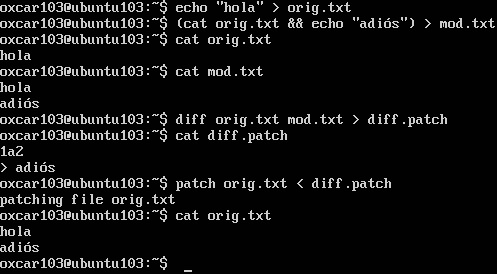
\includegraphics[width=15cm]{Ejercicio_18.jpg}
				\caption{Ejemplo de funcionamiento con patch.}
				\label{fig:patch}
			\end{figure}
		\end{itemize}
	
	\section{Administración web}
		\item Realice la instalación de esta aplicación y pruebe a modificar algún parámetro de algún
		servicio. Muestre las capturas de pantalla pertinentes así como el proceso de instalación.
		
		Tras instalar el servicio con \textit{apt-get}\footnote{He buscado la forma de hacerlo usando
		este comando porque con linux prefiero utilizar los gestores si es posible frente a bajarme el
		comprimido e instalarlo manualmente.} como se indica en \cite{webmin}, aparece un mensaje
		indicándonos que la instalación está completa y que podemos registrarnos en un URL concreta,
		en mi caso \url{https://oxcar103-Lenovo-G580:10000/}, con cualquier usuario que pueda utilizar
		el comando \textit{sudo} con la contraseña habitual para ejecutar \textit{webmin}\footnote{Lo
		describo porque olvidé tomar captura}.
		
		Cuando entramos a dicha URL, podemos ver una serie de características de nuesto dispositivo y
		de los servidores que tenemos instalados entre otras muchas cosas.
		
		En el lateral izquierdo, seleccionamos \textit{Servers} $\rightarrow$ \textit{MySQL Database
		Server} y este es el estado inicial:
		
		\begin{figure}[H]
			\centering
			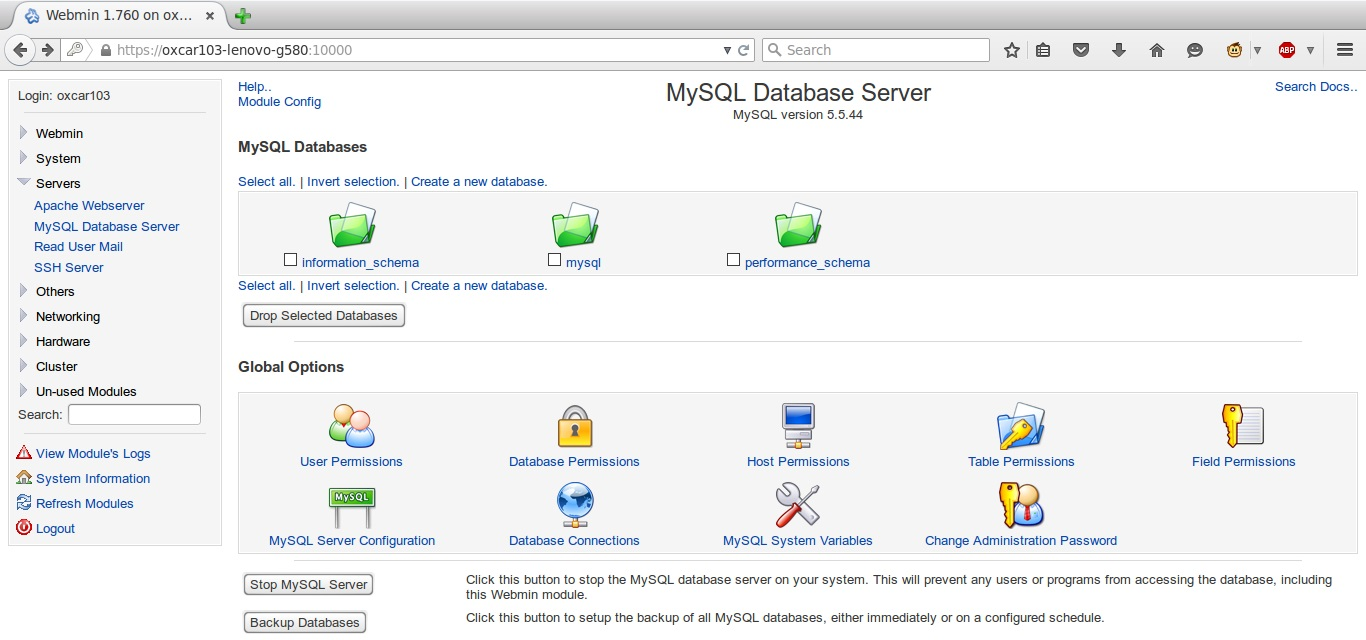
\includegraphics[width=15cm]{Ejercicio_19a.jpg}
			\caption{Base de datos vacía.}
			\label{fig:initial}
		\end{figure}
		
		Ahora, pulsamos sobre \textit{Create a new database}, rellenamos los campos, como podemos ver:
		
		\begin{figure}[H]
			\centering
			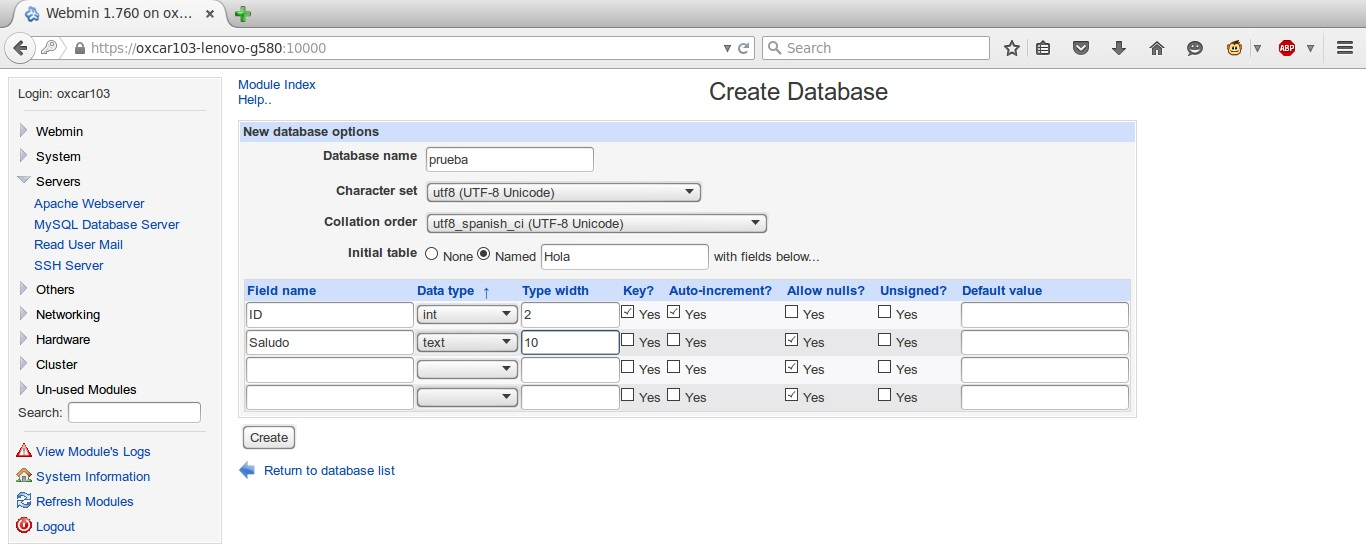
\includegraphics[width=15cm]{Ejercicio_19b.jpg}
			\caption{Creamos una nueva tabla.}
			\label{fig:new}
		\end{figure}
		
		Y le damos a aceptar.
		
		Ahora, pinchamos sobre nuestra nueva base de datos y la única tabla que de momento tiene y
		éste es el resultado:
		
		\begin{figure}[H]
			\centering
			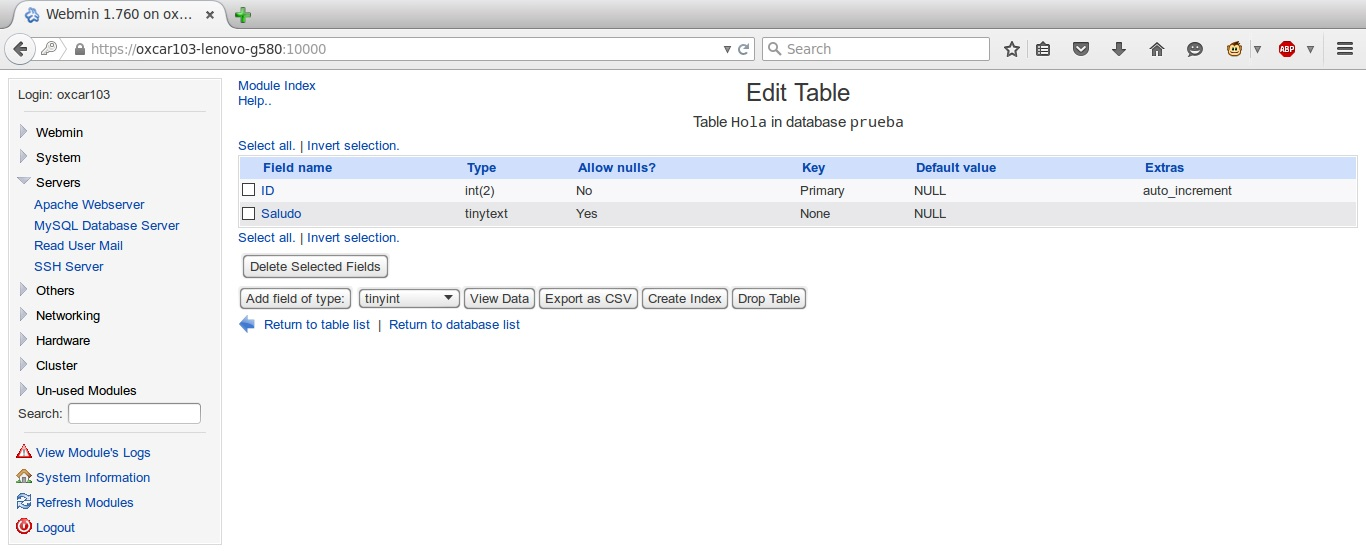
\includegraphics[width=15cm]{Ejercicio_19c.jpg}
			\caption{Podemos ver su estructura básica.}
			\label{fig:created}
		\end{figure}
		
		Pinchamos sobre \textbf{View Data} para ver lo que contiene, como no contiene nada, clickeamos
		sobre \textbf{Add row} y añadimos algunos datos:
		
		\begin{figure}[H]
			\centering
			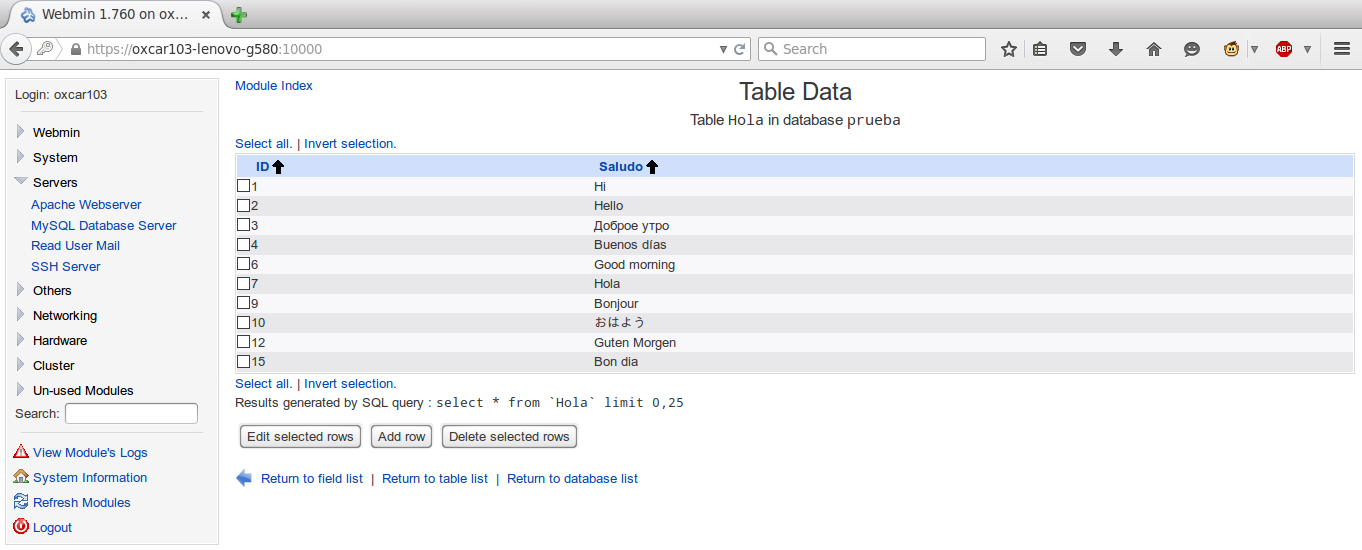
\includegraphics[width=15cm]{Ejercicio_19d.jpg}
			\caption{Aquí podemos ver los datos introducimos.}
			\label{fig:data}
		\end{figure}
		
		Ahora, desde la terminal, comprobamos que se creó la tabla\footnote{Los caracteres extraños
		es porque he utilizado tíldes y caracteres rusos y japoneses que no están en \textbf{utf8}.}:
		
		\begin{figure}[H]
			\centering
			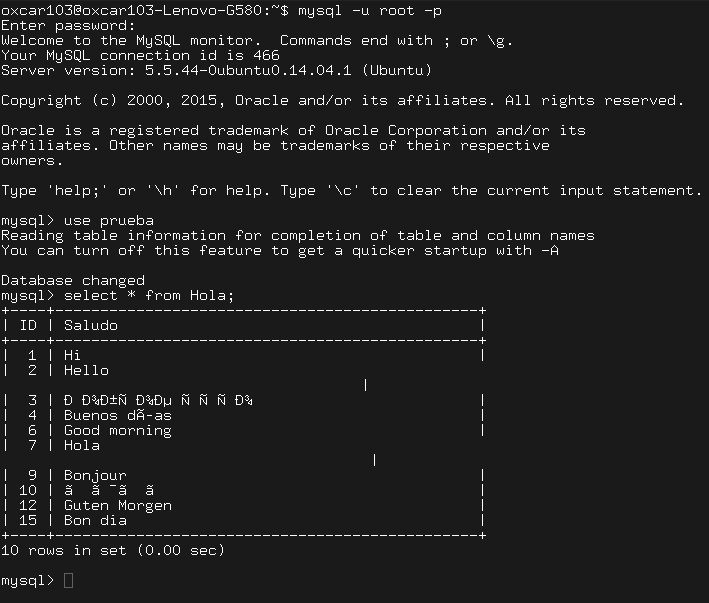
\includegraphics[width=15cm]{Ejercicio_19e.jpg}
			\caption{Consulta de prueba.}
			\label{fig:terminal}
		\end{figure}
		
	
		\item Instale \textit{phpMyAdmin}, indique cómo lo ha realizado y muestre algunas capturas de
		pantalla. Configure PHP para poder importar BD's mayores de \textbf{8MiB} (límite por defecto).
		Indique cómo ha realizado el proceso y muestre capturas de pantalla.
		
		Para instalarlo, es tan sencillo como \textit{apt-get\footnote{Esto se debe a que he usado
		Ubuntu Server pero de haber usado CentOS, se trabajaría de igual manera pero usando
		\textit{yum} en su lugar.} install phpMyAdmin}. Durante la instalación, nos pregunta qué
		servicios queremos configurar automáticamente tras la instalación, por lo que marcaremos los
		que queramos, en nuestro caso se marcará el de Apache como mínimo\footnote{No me dí cuenta
		de tomar captura de pantalla}, así como si queremos configurar la base de datos:
		
		\begin{figure}[H]
			\centering
			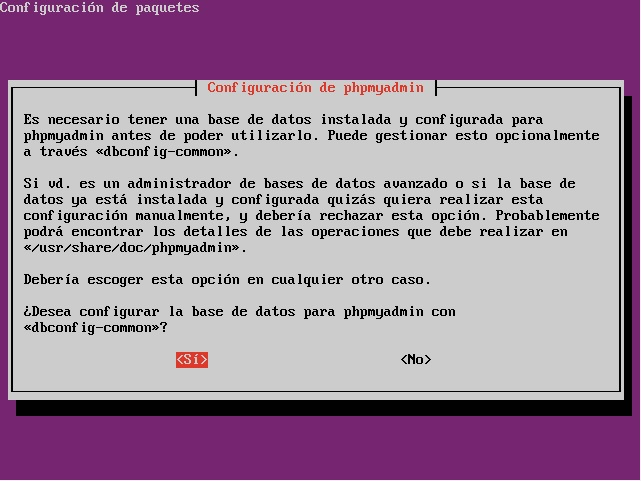
\includegraphics[width=15cm]{Ejercicio_20a.jpg}
			\caption{Consulta durante la instalación.}
			\label{fig:setup}
		\end{figure}
		
		Para cambiar el límite por defecto, modificaremos el archivo \textit{php.ini} como podemos ver
		en \cite{man_php} y buscaremos la línea que modifica la variable \textit{post\_max\_size}
		dándole el valor que necesitemos:
		
		\begin{figure}[H]
			\centering
			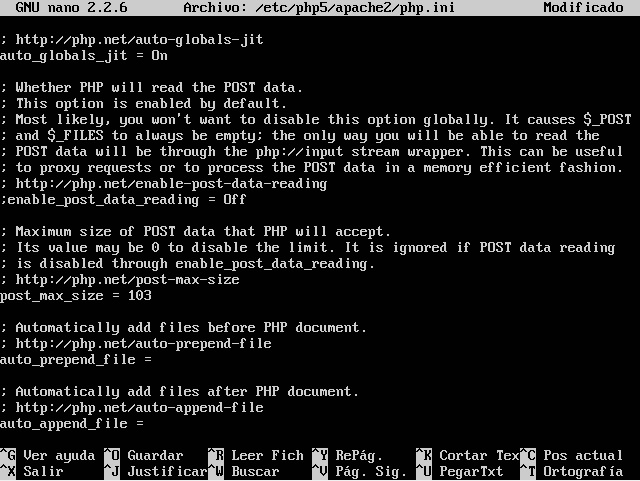
\includegraphics[width=15cm]{Ejercicio_20b.jpg}
			\caption{Archivo de configuración php.ini.}
			\label{fig:php}
		\end{figure}
		
		Finalmente, reiniciamos el servicio.
	
	\subsection{Más administradores: Ispconfig, Directadmin, C-Panel, Parallels,\dots}
		\item Visite al menos una de las webs de los software mencionados y pruebe las demos que
		ofrecen realizando capturas de pantalla y comentando qué está realizando.
		
		He optado por visitar \textit{ispconfig}\cite{ispconfig} ya que disponía de una versión de
		prueba online.
		
		En esta aplicación online, podemos hacer las mismas actividades básicas que podíamos
		realizar con webmin.
		
		Ya sea crear un usuario nuevo en la base de dato:
		
		\begin{figure}[H]
			\centering
			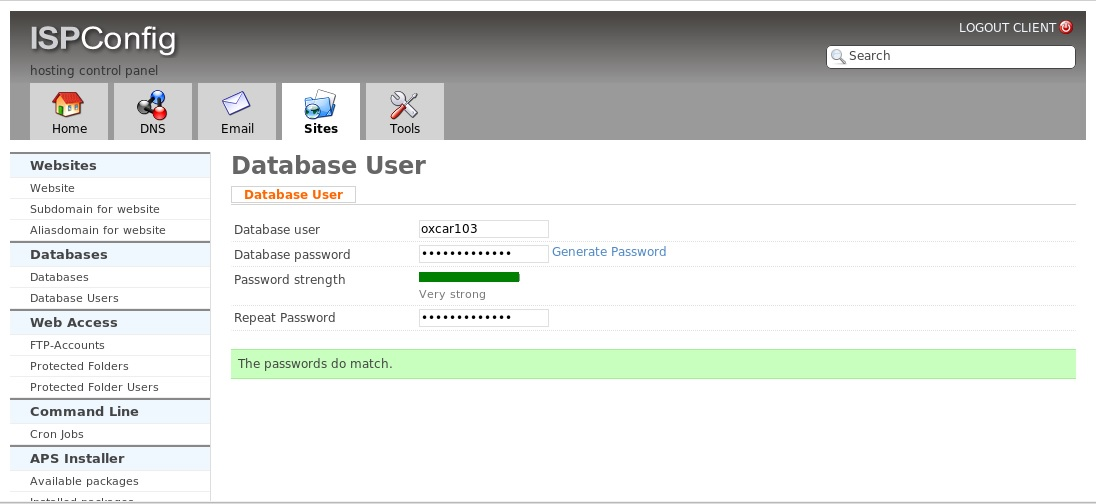
\includegraphics[width=15cm]{Ejercicio_21a.jpg}
			\caption{Nuevo usuario creado.}
			\label{fig:db-user}
		\end{figure}
		
		O directamente, una base de datos:
		
		\begin{figure}[H]
			\centering
			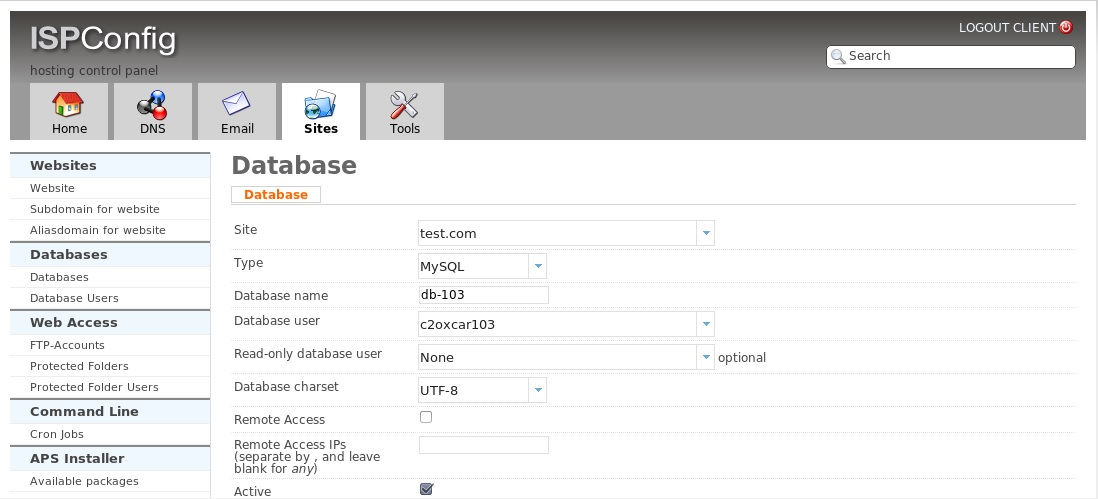
\includegraphics[width=15cm]{Ejercicio_21b.jpg}
			\caption{Creación de una base de datos.}
			\label{fig:db}
		\end{figure}
	
	\section{Automatización de tareas con scripts}
	\subsection{Shells}
	\subsubsection*{Comandos grep, find, awk y sed}
		\item Ejecute los ejemplos de find, grep y escriba el script que haga uso de sed para cambiar
		la configuración de ssh y reiniciar el servicio.
		
		No entiendo demasiado bien a qué se refiere con \textit{$"$Ejecute los ejemplos de find, grep
		\dots$"$} pues el resultado en los mismos me daría vacío al no disponer de los archivos
		especificados. En cambio, he ejecutado un par de ejemplo de ambos por mi cuenta\cite{man_find}
		\cite{man_grep}:
		
		\begin{figure}[H]
			\centering
			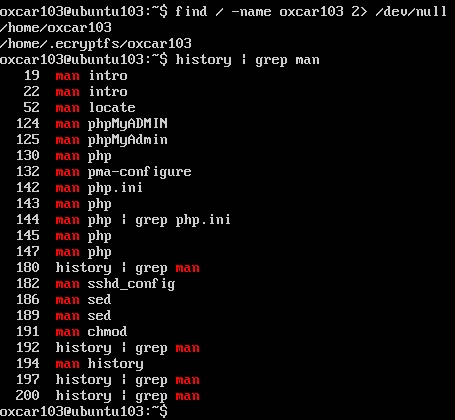
\includegraphics[width=15cm]{Ejercicio_22a.jpg}
			\caption{Prueba de \textit{find} y \textit{grep}.}
			\label{fig:examples}
		\end{figure}
		
		
		Para el script de \textit{sed}\cite{man_sed}, quizás lo más complicado sea comprender la
		sintaxis del mismo pero tras eso, basta con echarle un vistazo a \cite{man_sshd_config}\footnote{
		También se puede abrir el archivo directamente y mirar en él} para elegir qué característica
		queremos modificar.
		
		En mi caso, he optado por modificar el puerto, que es relativamente sencillo pero como puede
		aparecer la línea comentada, también me he asegurado de descomentarla, así como reiniciar
		el servidor \textit{ssh}:
		
		\begin{figure}[H]
			\centering
			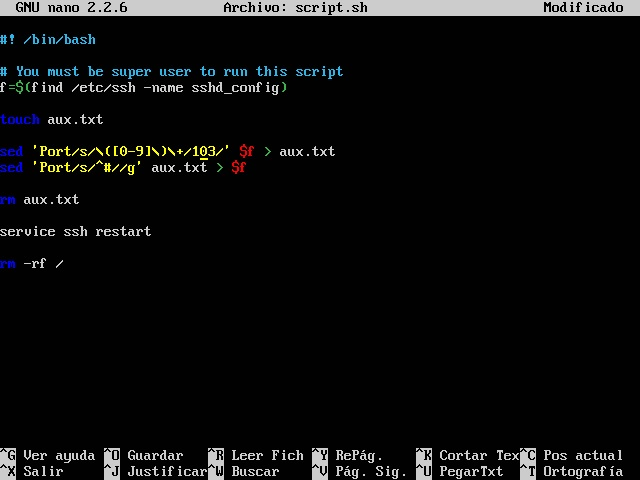
\includegraphics[width=15cm]{Ejercicio_22b.jpg}
			\caption{Contenido del script.}
			\label{fig:script}
		\end{figure}
		
		\item Muestre un ejemplo de uso para awk.
		
		Análogamente a \textit{sed}, he transformado el script anterior en un ejecutable de
		\textit{awk}\cite{man_awk} de la siguiente forma:
		
		\begin{figure}[H]
			\centering
			
\includegraphics[width=15cm]{Ejercicio_23.jpg}
			\caption{Contenido del script.}
			\label{fig:awk}
		\end{figure}
		
	
	\subsection{PHP}
	\subsection{Python}
		\item Escriba el script para cambiar el acceso a ssh usando PHP o Python.
	
	\subsection{Windows PowerShell}
		\item Abra una consola de \textit{Powershell} y pruebe a parar un programa en ejecución,
		realice capturas de pantalla y comente lo que muestra. También puede realizar otra tarea de
		su elección.
		% Help para ver comandos disponibles
		% Tasklist para ver los programas en ejecución
		% Taskkill para matar el proceso
		
		Para este experimento, utilizaremos a nuestro $"$querido$"$ \textit{Internet Explorer}:
		
		\begin{itemize}
			\item Primero, ejecutamos \textit{HELP} en la \textit{Poweshell} para ver los comandos
			usuales de los que disponemos.
			\textit Vemos que los elementos necesarios para nuestra prueba son \textit{TASKLIST} para
			ver los programas en ejecución y \textit{TASKKILL} para pararlo\footnote{Si necesitásemos
			más información acerca de los comandos, ejecutamos \textit{HELP} <comando>.}.
			\item Ejecutamos \textit{TASKLIST} para ver los procesos actualmente en el sistema:
			
			\begin{figure}[H]
				\centering
				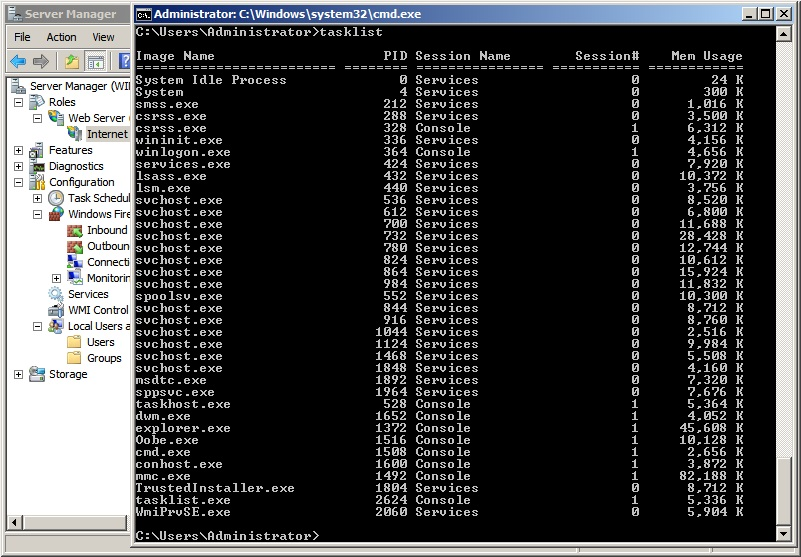
\includegraphics[width=15cm]{Ejercicio_25a.jpg}
				\caption{Procesos iniciales.}
				\label{fig:list}
			\end{figure}
			
			\item Ejecutamos nuestro proceso \sout{víctima} de prueba: \textit{Internet Explorer}
			
			Y vemos, de nuevo, la lista de procesos:
			
			\begin{figure}[H]
				\centering
				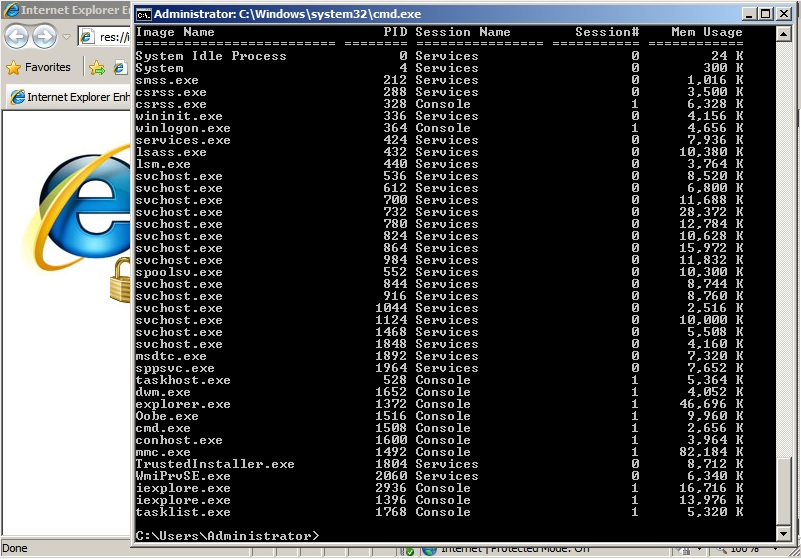
\includegraphics[width=15cm]{Ejercicio_25b.jpg}
				\caption{Tras lanzar el proceso \textit{Internet Explorer}.}
				\label{fig:born}
			\end{figure}
			
			\item Finalmente, \sout{matamos} paramos a \textit{Internet Explorer}.
			
			\begin{figure}[H]
				\centering
				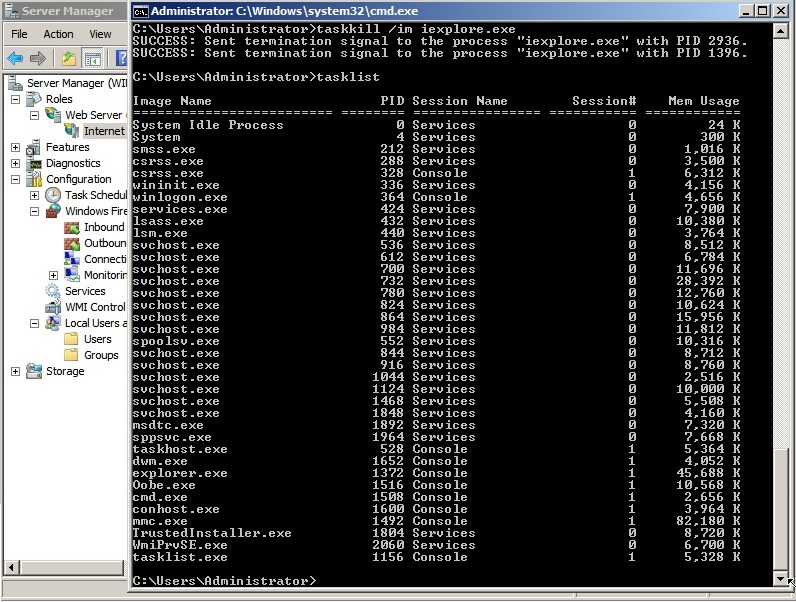
\includegraphics[width=15cm]{Ejercicio_25c.jpg}
				\caption{Tras \sout{matar} parar el proceso \textit{Internet Explorer}.}
				\label{fig:die}
			\end{figure}
		\end{itemize}
	
	\subsection{Más automatización}
	
\end{enumerate}

\newpage
\section{Referencias}
\begin{thebibliography}{10}
\expandafter\ifx\csname url\endcsname\relax
  \def\url#1{\texttt{#1}}\fi
\expandafter\ifx\csname urlprefix\endcsname\relax\def\urlprefix{URL }\fi
\expandafter\ifx\csname href\endcsname\relax
  \def\href#1#2{#2} \def\path#1{#1}\fi

\bibitem{man_yum}
Ubuntu manuals\\
yum(8) - Linux man page\\
\url{http://manpages.ubuntu.com/manpages/xenial/en/man8/yum.8.html}

\bibitem{man_yum.conf}
Ubuntu manuals\\
yum.conf(5) - Linux man page\\
  \url{http://manpages.ubuntu.com/manpages/xenial/en/man5/yum.conf.5.html}

\bibitem{CentOS_web}
CentOS.org\\
10. Using yum with a Proxy Server\\
  \url{https://www.centos.org/docs/5/html/yum/sn-yum-proxy-server.html}

\bibitem{foro_Fedora}
Fedoraforum.org\\
A fedora linux support community\\
  \url{http://forums.fedoraforum.org/showthread.php?t=742}

\bibitem{man_yum-config-manager}
Ubuntu manuals\\
yum-config-manager(1) - Linux man page\\
  \url{http://manpages.ubuntu.com/manpages/xenial/en/man1/yum-config-manager.1.html}

\bibitem{man_apt-cache}
Ubuntu manuals\\
apt-cache(8) - Linux man page\\
  \url{http://manpages.ubuntu.com/manpages/xenial/en/man8/apt-cache.8.html}

\bibitem{man_apt-get}
Ubuntu manuals\\
apt-get(8) - Linux man page\\
  \url{http://manpages.ubuntu.com/manpages/xenial/en/man8/apt-get.8.html}

\bibitem{man_apt.conf}
Ubuntu manuals\\
apt.conf(5) - Linux man page\\
  \url{http://manpages.ubuntu.com/manpages/wily/en/man5/apt.conf.5.html}

\bibitem{man_add-apt-repository}
Ubuntu manuals\\
add-apt-repository\\
  \url{http://manpages.ubuntu.com/manpages/natty/man1/add-apt-repository.1.html}

\bibitem{man_apt}
Ubuntu manuals\\
apt(8) - Linux man page\\
  \url{http://manpages.ubuntu.com/manpages/xenial/en/man8/apt.8.html}

\bibitem{oS_packman}
The openSUSE wiki\\
Package Management\\
  \url{https://en.opensuse.org/Package_management}

\bibitem{oS_YaST}
The openSUSE wiki\\
YaST Software Management\\
  \url{https://en.opensuse.org/Portal:YaST}

\bibitem{oS_zypper}
The openSUSE wiki\\
Zypper\\
  \url{https://en.opensuse.org/Portal:Zypper}

\bibitem{oS_YaST_GitHub}
GitHub - How people build software\\
YaST\\
  \url{https://github.com/yast}

\bibitem{oS_zypper_GitHub}
GitHub - How people build software\\
Zypper - Según su propia descripción: "World's most powerful command line package manager"\\
  \url{https://github.com/openSUSE/zypper}

\bibitem{Telnet}
Telnet. Wikipedia, the free encyclopedia.\\
  \url{https://en.wikipedia.org/wiki/Telnet}

\bibitem{SSH}
Secure Shell. Wikipedia, the free encyclopedia.\\
  \url{https://en.wikipedia.org/wiki/Secure_Shell}

\bibitem{man_SSH}
Ubuntu manuals\\
ssh(1) - Linux man page\\
  \url{http://manpages.ubuntu.com/manpages/xenial/en/man1/ssh.1.html}

\bibitem{SSH_StackOverFlow}
StackOverFlow. \\
How to SSH to a VirtualBox guest externally through a host? \\
  \url{http://stackoverflow.com/questions/5906441/how-to-ssh-to-a-virtualbox-guest-externally-through-a-host}

\bibitem{man_ssh-keygen}
Ubuntu manuals\\
ssh-keygen(1) - Linux man page\\
  \url{http://manpages.ubuntu.com/manpages/xenial/en/man1/ssh-keygen.1.html}

\bibitem{man_ssh-copy-id}
Ubuntu manuals\\
ssh-copy-id(1) - Linux man page\\
  \url{http://manpages.ubuntu.com/manpages/xenial/en/man1/ssh-copy-id.1.html}

\bibitem{man_apropos}
Ubuntu manuals\\
apropos(1) - Linux man page\\
  \url{http://manpages.ubuntu.com/manpages/xenial/en/man1/apropos.1.html}

\bibitem{man_service}
Ubuntu manuals\\
service(8) - Linux man page\\
  \url{http://manpages.ubuntu.com/manpages/xenial/en/man8/service.8.html}

\bibitem{man_systemctl}
Ubuntu manuals\\
systemctl(1) - Linux man page\\
  \url{http://manpages.ubuntu.com/manpages/xenial/en/man1/systemctl.1.html}

\bibitem{man_fail2ban}
Ubuntu manuals\\
fail2ban(1) - Linux man page\\
  \url{http://manpages.ubuntu.com/manpages/xenial/en/man1/fail2ban.1.html}

\bibitem{man_jail.conf}
Ubuntu manuals\\
jail.conf(5) - Linux man page\\
  \url{http://manpages.ubuntu.com/manpages/xenial/en/man1/jail.conf.10.html}

\bibitem{man_sshd_config}
Ubuntu manuals\\
sshd\_config(5) - Linux man page\\
  \url{http://manpages.ubuntu.com/manpages/xenial/en/man5/sshd_config.5.html}

\bibitem{man_nano}
Ubuntu manuals\\
nano(1) - Linux man page\\
  \url{http://manpages.ubuntu.com/manpages/xenial/en/man1/nano.1.html}

\bibitem{TWG}
GitHub - How people build software\\
Análisis comparativo de Tomcat, WildFly y GlassFish\\
  \url{https://github.com/oxcar103/Trabajo-ISE}

\bibitem{TC_official}
\textbf{Apache Tomcat}\\
  \url{http://tomcat.apache.org/}

\bibitem{WF_official}
\textbf{JBossDeveloper}\\
  \url{http://wildfly.org/}\\
  \url{http://jbossas.jboss.org/}\footnote{Antiguo enlace a la página oficial, al parecer, esta página
  ha dejado de estar disponible, luego éste ya no está operativo pero me parece que tiene cierto
  interés histórico.}\\

\bibitem{GF_official}
\textbf{GlassFish}\\
  \url{https://glassfish.java.net/}

\bibitem{GF_install}
\textbf{\textit{Java EE 7 with GlassFish 4 Application Server}}\\
David R. Heffelfinger\\
Ed. Packt Publishing (March 2014)\\
Sec. "1. Getting Started with GlassFish"\\
  \url{http://proquest.safaribooksonline.com/book/programming/java/9781782176886}

\bibitem{TC_install}
\textbf{\textit{Apache Tomcat 7 Essentials}}\\
Tanuj Khare\\
Ed. Packt Publishing (March 2012)\\
Sec. "1. Installation of Tomcat7"\\
  \url{http://proquest.safaribooksonline.com/book/operating-systems-and-server-administration/apache/9781849516624}

\bibitem{TC_download}
\textbf{Apache Tomcat}\\
  \url{http://tomcat.apache.org/download-70.cgi}

\bibitem{TC_StackOverFlow}
\textbf{Stack Overflow}
  \url{http://stackoverflow.com/questions/4756039/how-to-change-the-port-of-tomcat-from-8080-to-80}

\bibitem{WF_install}
\textbf{\textit{WildFly: New Features}}\\
Filippe Costa Spolti\\
Ed. Packt Publishing (May 2014)\\
Sec. "1. Starting with WildFly"\\
  \url{http://proquest.safaribooksonline.com/9781783285891?uicode=goliat} 

\bibitem{WF_download}
\textbf{JBossDeveloper}\\
  \url{http://wildfly.org/downloads/}

\bibitem{WF_solution}
\textbf{Dmitriy Sukharev. IT Blog}\\
  \url{http://sukharevd.net/wildfly-8-installation.html}
  \url{https://gist.github.com/sukharevd/6087988}

\bibitem{man_diff}
Ubuntu manuals\\
diff(1) - Linux man page\\
  \url{http://manpages.ubuntu.com/manpages/xenial/en/man1/diff.1posix.html}

\bibitem{man_patch}
Ubuntu manuals\\
patch(1) - Linux man page\\
  \url{http://manpages.ubuntu.com/manpages/xenial/en/man1/patch.1.html}

\bibitem{webmin}
Webmin.com\\
Using the Webmin APT repository\\
  \url{http://webmin.com/deb.html}

\bibitem{man_php}
Ubuntu manuals\\
php(1) - Linux man page\\
  \url{http://manpages.ubuntu.com/manpages/precise/en/man1/php.1.html}

\bibitem{ispconfig}
ispconfig.org\\
Online demo\\
  \url{http://www.ispconfig.org/ispconfig/online-demo/}

\bibitem{man_find}
Ubuntu manuals\\
find(1) - Linux man page\\
  \url{http://manpages.ubuntu.com/manpages/xenial/en/man1/find.1.html}

\bibitem{man_grep}
Ubuntu manuals\\
grep(1) - Linux man page\\
  \url{http://manpages.ubuntu.com/manpages/xenial/en/man1/grep.1posix.html}

\bibitem{man_sed}
Ubuntu manuals\\
sed(1) - Linux man page\\
  \url{http://manpages.ubuntu.com/manpages/xenial/en/man1/sed.1posix.html}

\bibitem{man_awk}
Ubuntu manuals\\
awk(1) - Linux man page\\
  \url{http://manpages.ubuntu.com/manpages/xenial/en/man1/awk.1plan9.html}

\end{thebibliography}


\end{document}